\section{Are there grandmother cells in CNNs?}
In the main paper we studied the nature of representations in mid-level CNN representations given by conv-5. Here, we address the same question for layer fc-7, which is the last layer of CNN and features extracted from this lead to best performance. The results for number of filters required to achieve the same performance as all the filters taken together is presented in Figure \ref{fig:svm-sel-dims}. Table \ref{table:num-fil} reports the number of filters required per class to obtain 50\% and 90\% of the complete performance. It can be seen that like conv-5, feature representations in fc-7 are also distributed for a large number of classes. It is interesting to note, that for most classes 50\% performance can be reached using a single filter, but for reaching 90\% performance a lot more filters are required. 
\setlength{\unitlength}{\linewidth}
\begin{figure}[t!]
\centering
%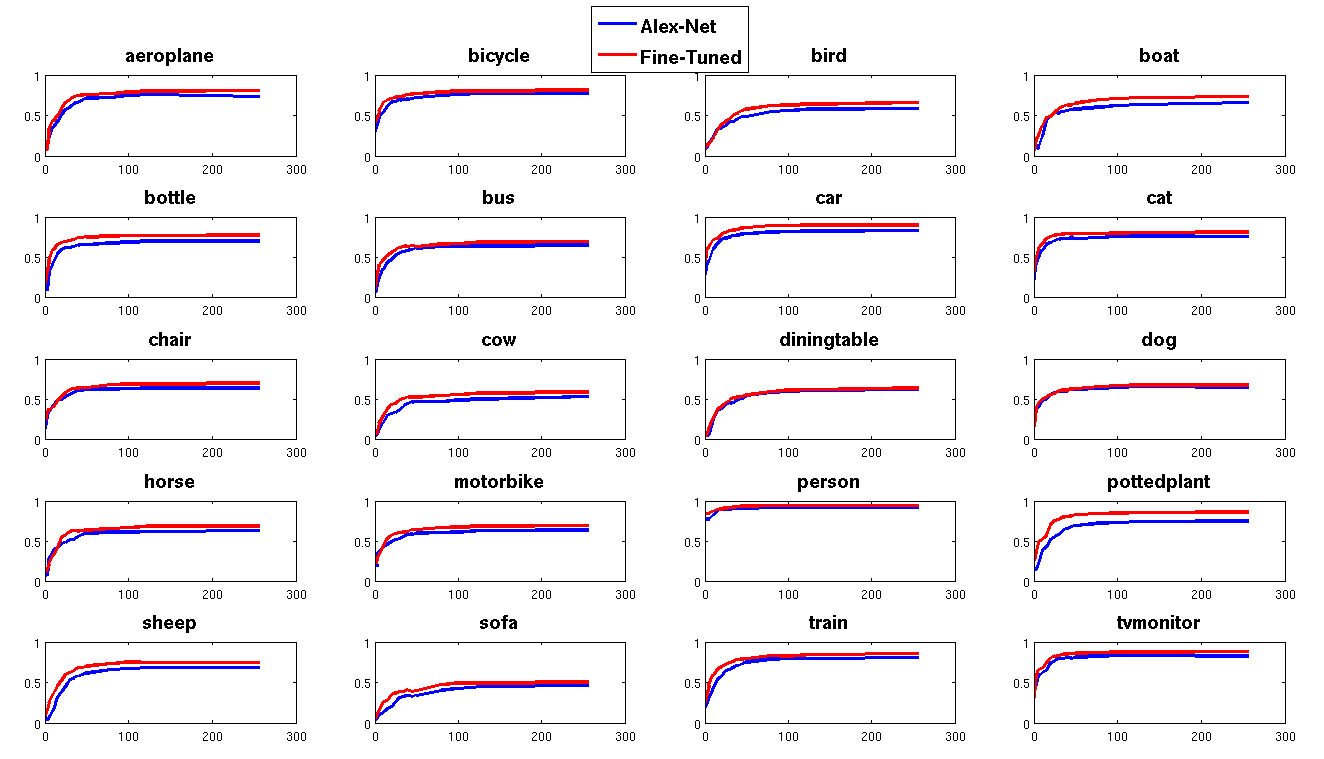
\includegraphics[height=6.5cm]{images/svm_seldims.png}
\begin{picture}(0.04,0.3)(0,0)
\put(0.0,0.1){\rotatebox{90}{\scriptsize{\textbf{Fraction of complete performance}}}}
\end{picture}
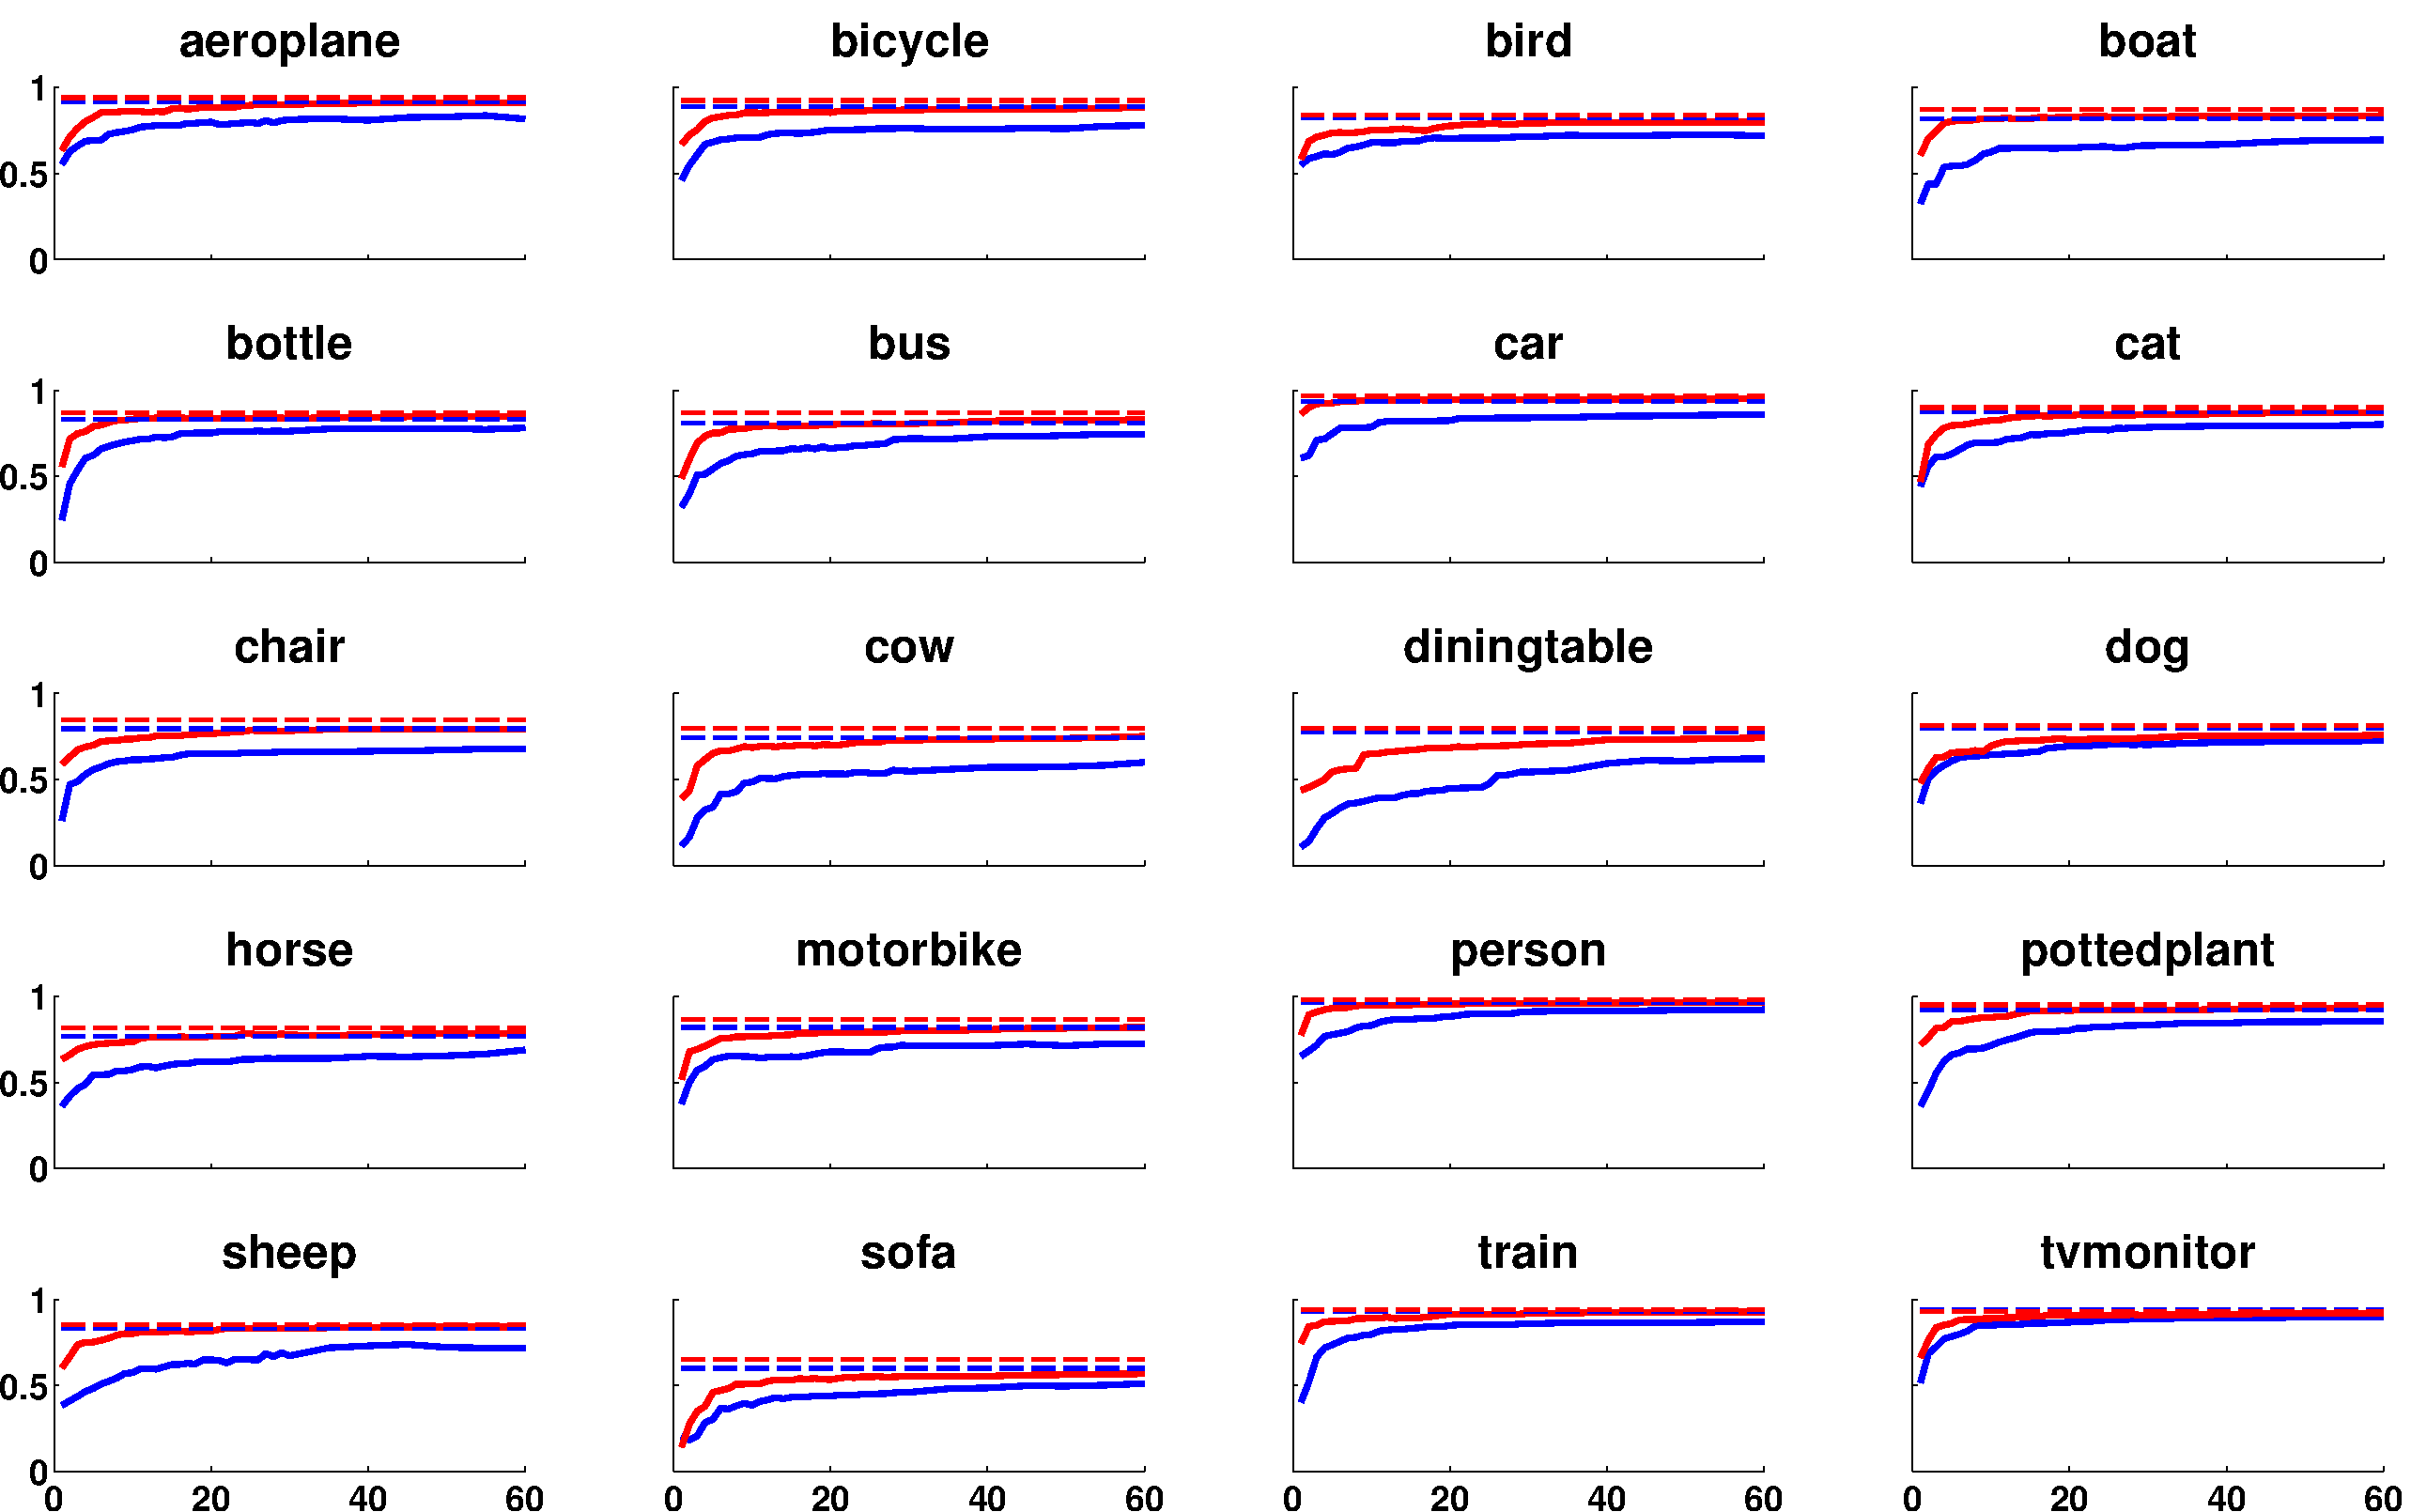
\includegraphics[width=0.93\linewidth]{images/relu7_svm_filters.pdf}
\begin{picture}(1.0,0.01)(0,0)
\put(0.40,0.0){{\scriptsize{\textbf{Number of fc-7 filters}}}}
\end{picture}
\caption{The fraction of complete performance on PASCAL-DET-GT achieved by fc-7 filter subsets of different sizes. Complete performance is the AP computed by considering responses of all the filters. The solid blue and red lines are for pre-trained and fine-tuned network respectively. The dashed blue and red lines show the complete performance.  Notice, that for a few classes such as person, bicycle and cars only a few filters are required, but for many classes substantially more filters are needed, indicating a distributed code.}
\label{fig:svm-sel-dims}
\end{figure}  

\setlength{\tabcolsep}{1.1pt}
\begin{table}[t!]
\renewcommand{\arraystretch}{1.2}
\begin{center}
\caption{Number of filters required to achieve 50\% or 90\% of the complete performance on PASCAL-DET-GT using a CNN pre-trained on ImageNet and fine-tuned for PASCAL-DET using fc-7 features.}
\label{table:num-fil}
\resizebox{\linewidth}{!}{
\begin{tabular}{l|c||cccccccccccccccccccc}
\noalign{\smallskip}
& perf. & aero & bike & bird & boat & bottle & bus & car & cat & chair & cow & table & dog & horse & mbike & person & plant & sheep & sofa & train & tv \\
\hline
pre-train & 50\% & 1 & 1 & 1 & 2 & 2 & 3 & 1 & 1 & 2 & 6 & 11 & 2 & 2 & 2 & 1 & 3 & 3 & 5 & 2 & 1 \\
fine-tune & 50\% & 1 & 1 & 1 & 1 & 1 & 1 & 1 & 1 & 1 & 2 & 1 & 1 & 1 & 1 & 1 & 1 & 1 & 3 & 1 & 1 \\
\hline
pre-train & 90\% & 33 & 40 & 40 & 40 & 17 & 32 & 32 & 31 & 40 & 40 & 40 & 35 & 37 & 37 & 17 & 29 & 40 & 40 & 17 & 8\\
fine-tune & 90\% & 6 & 7 & 11 & 4 & 5 & 10 & 2 & 8 & 19 & 27 & 32 & 18 & 9 & 16 & 2 & 7 & 7 & 40 & 3 & 4 
\end{tabular}
}
\end{center}
\end{table}
\setlength{\tabcolsep}{1.4pt}
